\chapter {Algorithm Design}

%have each subroutine listed with subroutine name as section then subsecs for flowchart, intital code, debugging and testing etc.
After planning my traffic light control system, I can now begin to design the algorithms. Looking at the exam board template provided to us, it is clear that the microcontroller can run subroutines as well as a procedural main program code section. \newline
Using subroutines is the most efficient way to program as it allows you to use the same lines of code a number of times, not only does this reduce the total number of lines of code you have to program but it also reduces the number of lines of code which are flashed onto the microcontroller. Using this knowledge, I designed my main program to call a number of subroutines. \newline

\noindent \textit{Shown below are the flowcharts and initial iteration of the algorithms. Full code listings are available in Appendix \ref{app:full-code}. Testing and debugging of the code is available in Chapter \ref{chap:testing}.}


\section{Main Program}
This code gets run automatically once the microcontroller has initialised. \newline
\noindent This algorithm works by initialising the stop LEDs by turning them all on. It then sequentially cycles through all of the sets of traffic lights, allowing them to cycle each time. After each set of traffic lights, it runs the \verb|checkPedstrian| algorithm which will check if there are pedestrians waiting to cross. This cycle repeats until the system is powered down.
\subsection*{Flowchart}
\begin{figure}[H]
    \centering
    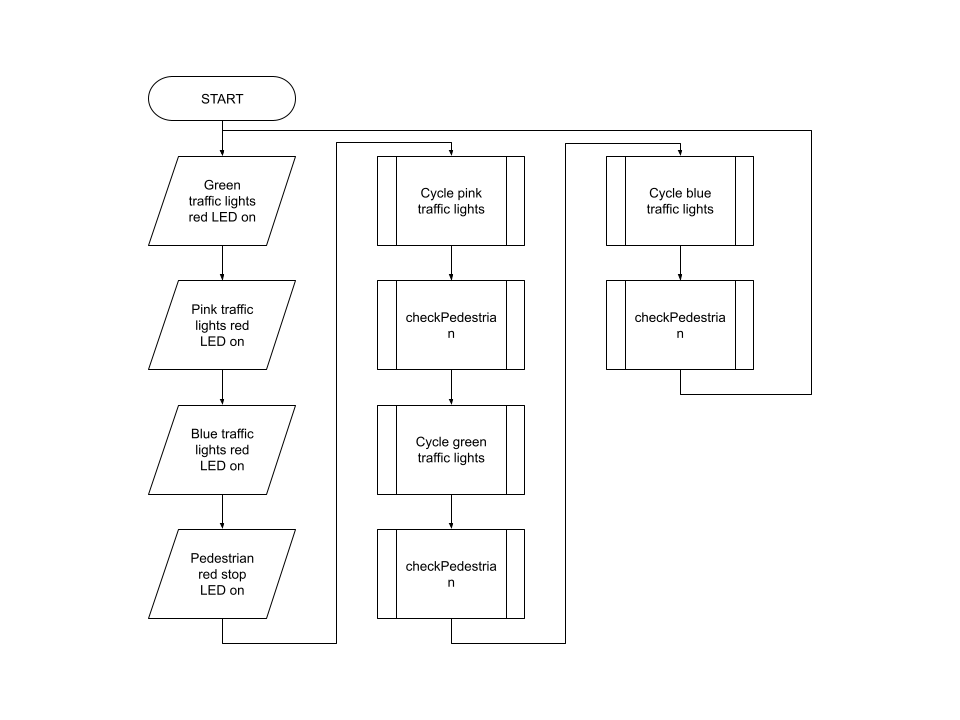
\includegraphics[width=0.9\textwidth]{images/flowchart-main.png}
    \caption{Main program flowchart}
    \label{fig:flowchart-main}
\end{figure}
\subsection*{Code}
\begin{lstlisting}[language={[x86masm]Assembler}, style=assembly, caption=Main sequence code]
;first turn on all stop leds
	bsf PORTA, 0 ;turn on pink set stop eld
	bsf PORTA, 3 ;turn on green set stop led
	bsf PORTA, 6 ;turn on blue set stop led
	bsf PORTB, 3 ;turn on pedestrian stop led

mtop call pinkTrafficLightSequence
	call checkPedestrian
	call greenTrafficLightSequence
	call checkPedestrian
	call blueTrafficLightSequence
	call checkPedestrian
	goto mTop
\end{lstlisting}

\section{checkButton Subroutine}
This algorithm is used to check if the pedestrian button has been pressed and if it has, turn on the red wait LED which would be found at traffic lights with pedestrian crossings.

\subsection*{Flowchart}
\begin{figure}[H]
    \centering
    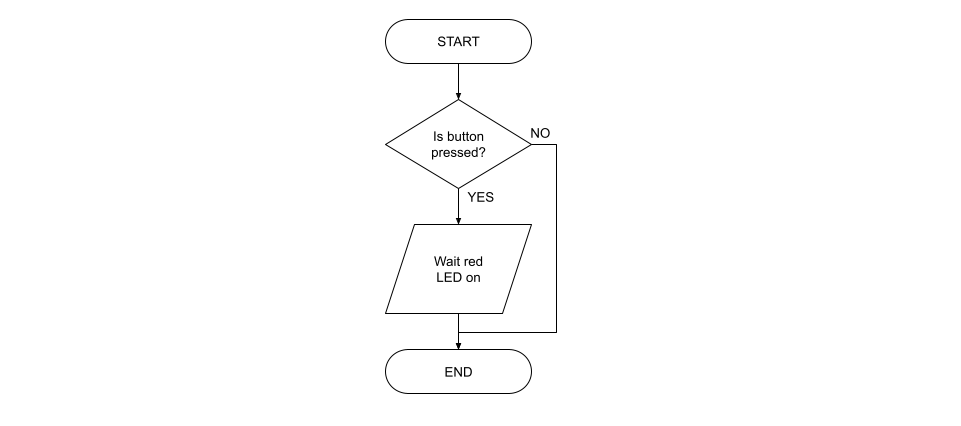
\includegraphics[width=0.9\textwidth]{images/flowchart-checkButton.png}
    \caption{Check button subroutine flowchart}
    \label{fig:flowchart-checkButton}
\end{figure}
\subsection*{Code}
\begin{lstlisting}[language={[x86masm]Assembler}, style=assembly, caption=checkButton subroutine]
;function to check the button
checkButton
	btfss PORTB, 1 ;skip next line of code if button pressed (active high)
	return ;can go back to where called from
	bsf PORTB, 2 ;turn red wait LED on
	return ;go back to main code
;end of function
\end{lstlisting}

\section{checkPedestrian Subroutine}
This algorithms is used to read the current state of the pedestrian wait LED. Depending on this state, it will either return straight to the main code or run the \verb|cyclePedestrian| subroutine.

\subsection*{Flowchart}
\begin{figure}[H]
    \centering
    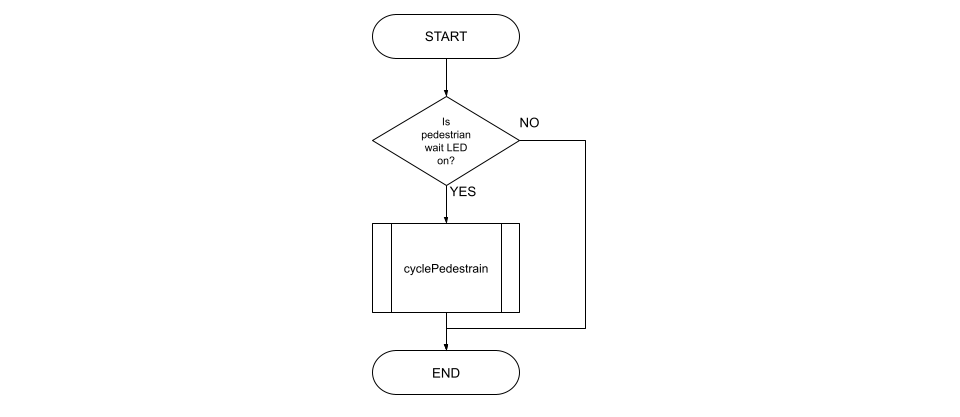
\includegraphics[width=0.9\textwidth]{images/flowchart-checkPedestrian.png}
    \caption{checkPedestrain subroutine flowchart}
    \label{fig:flowchart-chechPedestrian}
\end{figure}
\subsection*{Code}
\begin{lstlisting}[language={[x86masm]Assembler}, style=assembly, caption=checkPedestrian subroutine]
checkPedestrian
	;function to check if the wait led is on
		;if yes - cycle pedestrian crossing
		;if no - return to main 
	btfsc PORTB, 2 ;skip next line if wait led NOT on therefore if on, run next line
	call cycleCrossing
	return
;end function
\end{lstlisting}

\section{cycleCrossing Subroutine}
This algorithm will control the pedestrian crossing to allow the pedestrians to cross. 
\subsection*{Flowchart}
\begin{figure}[H]
    \centering
    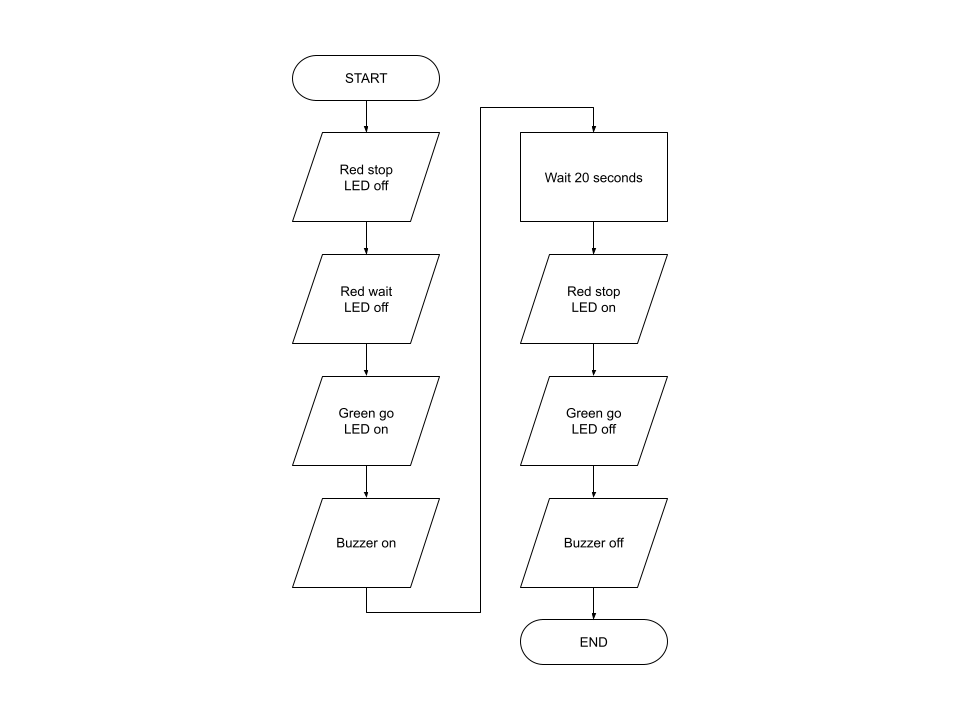
\includegraphics[width=0.9\textwidth]{images/flowchart-pedCrossingCycle.png}
    \caption{cycleCrossing subroutine flowchart}
    \label{fig:flowchart-cyclePedCrossing}
\end{figure}
\subsection*{Code}
\begin{lstlisting}[language={[x86masm]Assembler}, style=assembly, caption=cycleCrossing subroutine]
; function to cycle the pedestrian crossing
cycleCrossing
	bcf PORTB, 2 ;turn off red wait LED
	bcf PORTB, 3 ;turn off red stop LED
	bsf PORTB, 4 ;turn on green go LED
	bsf PORTB, 5 ;turn on buzzer
	call wait1000ms ;wait 1second
	call wait1000ms ;wait 1second
	call wait1000ms ;wait 1second
	call wait1000ms ;wait 1second
	call wait1000ms ;wait 1second
	call wait1000ms ;wait 1second
	call wait1000ms ;wait 1second
	call wait1000ms ;wait 1second
	call wait1000ms ;wait 1second
	call wait1000ms ;wait 1second
	call wait1000ms ;wait 1second
	call wait1000ms ;wait 1second
	call wait1000ms ;wait 1second
	call wait1000ms ;wait 1second
	call wait1000ms ;wait 1second
	call wait1000ms ;wait 1second
	call wait1000ms ;wait 1second
	call wait1000ms ;wait 1second
	call wait1000ms ;wait 1second
	call wait1000ms ;wait 1second
	;now have waited 20seconds so invert things and return to main sequence
	bcf PORTB, 4 ;turn off green go LED
	bsf PORTB, 3 ;turn on red stop LED
	bcf PORTB, 5 ;turn off buzzer
	return ;return to the main program
;end of function
\end{lstlisting}

\section{wait5SecondsCheckButton Subroutine}
This algorithm is much more complicated that I originally anticipated it to be. What I wanted it to do was to wait 10ms then run the \verb|checkButton| subroutine. To do this, I would have a loop which counted to 500. This is not possible using this PIC microcontroller as it has a maximum number size of 256. To get around this, I am using two loops, X and Y. This will allow me to wait for five seconds and every 10ms of that, check if the button is pressed or not.
\subsection*{Flowchart}
\begin{figure}[H]
    \centering
    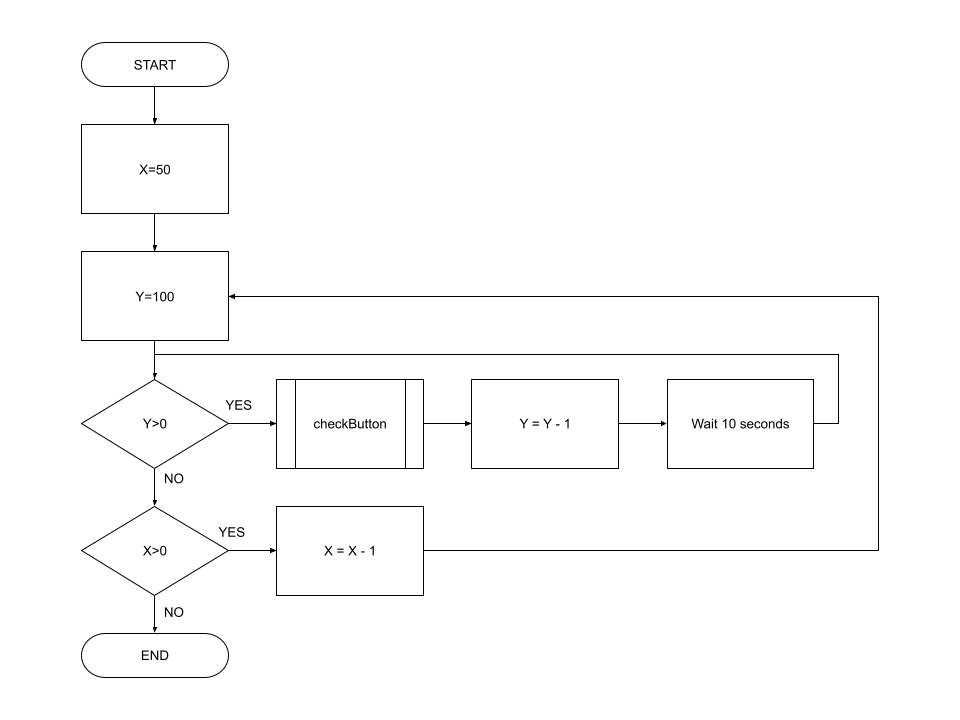
\includegraphics[width=0.9\textwidth]{images/flowchart-wait5Sec.png}
    \caption{wait5SecondsCheckButton subroutine flowchart}
    \label{fig:flowchart-wait5Sec}
\end{figure}
\subsection*{Code}
\begin{lstlisting}[language={[x86masm]Assembler}, style=assembly, caption=wait5SecondsCheckButton subroutine]
waitFiveSecondsCheckButton
	;first, stary loop x
	movlw d'51' ;set val of 51 into w register
	movf loopX ; move the val in the working register (51) into loopX

topX decfsz loopX, 1 ;decrement loopX and place the new value back into loopX
	goto startY ;line skipped if result is 0
	return

startY movlw d'101'; ;set value of 101 into w register
	movf loopY ;move value in working register (101) into loopY

topY decfsz loopY, 1 ;decrement loopY and place new value back into loopY
	goto finalPart ;goto final part of the function
	goto startX ;run if loopY = 0

finalPart call checkButton
	call wait10ms ;wait for 10ms function
	goto startY ;go back up to startY and loop around again
;end of function
\end{lstlisting}

\section{Traffic lights}
The traffic light control algorithm is fundamentally the same for the three sets of traffic lights. This is shown in the flowchart, as there is only one for the three subroutines. The only difference between the three sets is which IO bits are changed.
\subsection*{Flowchart}
\begin{figure}[H]
    \centering
    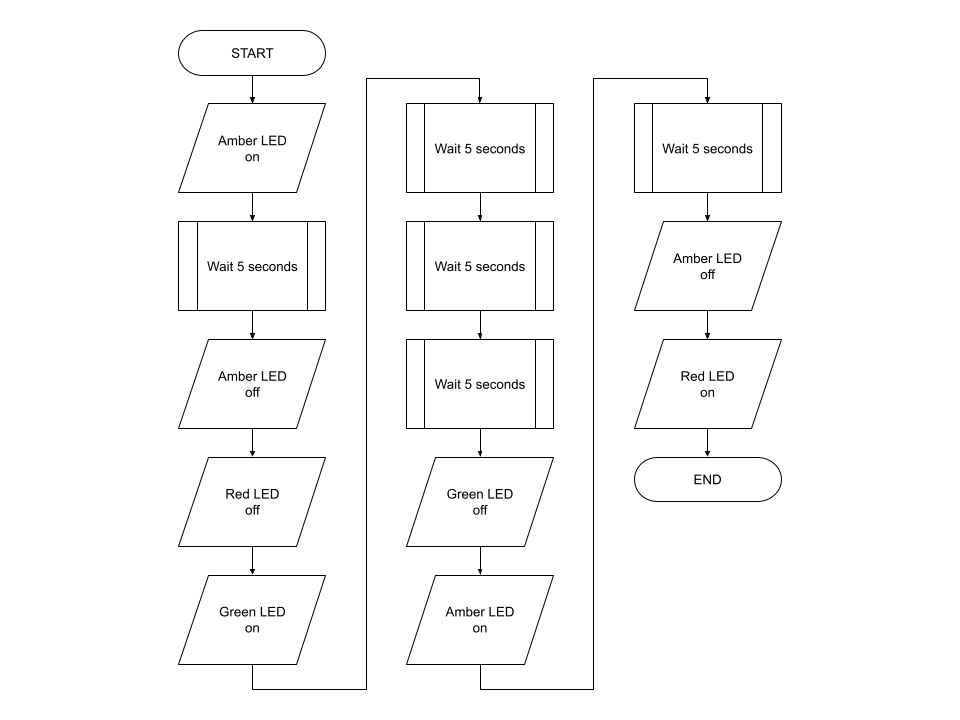
\includegraphics[width=0.9\textwidth]{images/flowchart-trafficLights.png}
    \caption{trafficLights subroutine flowchart}
    \label{fig:flowchart-trafficLights}
\end{figure}

\subsection*{Code}
\subsubsection*{Pink set}
\begin{lstlisting}[language={[x86masm]Assembler}, style=assembly, caption=Pink Traffic Light sequence]
pinkTrafficLightSequence
	bsf PORTA, 1 ;turn on amber led
	call waitFiveSecondsCheckButton ;wait 5s
	bcf PORTA, 1 ;turn off amber led
	bcf PORTA, 0 ;turn off red led
	bsf PORTA, 2 ; turn on greeen led
	call waitFiveSecondsCheckButton
	call waitFiveSecondsCheckButton
	call waitFiveSecondsCheckButton
	bcf PORTA, 2 ;turn off green led
	bsf PORTA, 1 ;turn on amber led
	call waitFiveSecondsCheckButton
	bsf PORTA, 0 ;turn on red led
	bcf PORTA, 1 ;turn off amber led
	return ;go back to main code
;end of function
\end{lstlisting}
\subsubsection*{Green set}
\begin{lstlisting}[language={[x86masm]Assembler}, style=assembly, caption=Green Traffic Light sequence]
greenTrafficLightSequence
	bsf PORTA, 4 ;turn on amber led
	call waitFiveSecondsCheckButton ;wait 5s
	bcf PORTA, 4 ;turn off amber led
	bcf PORTA, 3 ;turn off red led
	bsf PORTA, 5 ; turn on greeen led
	call waitFiveSecondsCheckButton
	call waitFiveSecondsCheckButton
	call waitFiveSecondsCheckButton
	bcf PORTA, 5 ;turn off green led
	bsf PORTA, 4 ;turn on amber led
	call waitFiveSecondsCheckButton
	bsf PORTA, 3 ;turn on red led
	bcf PORTA, 4 ;turn off amber led
	return ;go back to main code
;end of function
\end{lstlisting}

\subsubsection*{Blue set}
\begin{lstlisting}[language={[x86masm]Assembler}, style=assembly, caption=Blue Traffic Light sequence]
blueTrafficLightSequence
	bsf PORTA, 7 ;turn on amber led
	call waitFiveSecondsCheckButton ;wait 5s
	bcf PORTA, 7 ;turn off amber led
	bcf PORTA, 6 ;turn off red led
	bsf PORTB, 0 ; turn on greeen led
	call waitFiveSecondsCheckButton
	call waitFiveSecondsCheckButton
	call waitFiveSecondsCheckButton
	bcf PORTB, 0 ;turn off green led
	bsf PORTA, 7 ;turn on amber led
	call waitFiveSecondsCheckButton
	bsf PORTA, 6 ;turn on red led
	bcf PORTA, 7 ;turn off amber led
	return ;go back to main code
;end of function
\end{lstlisting}